\documentclass[a4paper,12pt]{book}

\usepackage[T2A]{fontenc}

% локаль
\usepackage[utf8]{inputenc}

% русский язык с переносами
\usepackage[english,russian]{babel}

% вставка картинок
\usepackage{graphicx}  

% настроим префиксы к рисункам (вместо "фиг." используем "рис")
\usepackage{caption}
\captionsetup[figure]{name=рис.}
\captionsetup[table]{name=таб.}

% Дополнительная работа с таблицами
\usepackage{array,tabularx,tabulary,booktabs}

% пригодится для формул
\usepackage{amsfonts,amssymb,amsthm,mathtools}
\usepackage{amsmath}

\usepackage{wrapfig}
\usepackage{float}

\begin{document}

Пусть рис. \ref{fig:noname_1} представляет положение Солнца $S$, Земли $T$ и Луны $L$, и путь $\Theta$ есть центр тяжести Земли и Луны. Делаем следующие обозначения:

\begin{table}[ht] %
	\centering
	\begin{tabular}{|l|c|}
		\hline
		Масса Солнца & $S$ \\
		\hline
		Масса Земли & $T$ \\
		\hline
		Масса Луны & $L$ \\
		\hline
	\end{tabular}
	\caption{Таблица условных обозначений}
	\label{tbl:1}
\end{table}

Расстояние:
\[ S\Theta=\rho;\ ST=\rho_1;\ SL=\rho_2;\ TL=r\]
тогда будет:
%
\begin{equation}
	\begin{aligned}
		T\Theta=r_1=\frac{L}{T+L}\cdot r \\
		L\Theta=r_2=\frac{T}{T+L}\cdot r
	\end{aligned}
	\label{eq:1}
\end{equation}

Составим теперь выражения ускорений, которые эти тела сообщают друг другу.

\begin{wrapfigure}{l}{0.5\textwidth}
	\vspace{-20pt}
	\begin{center}
		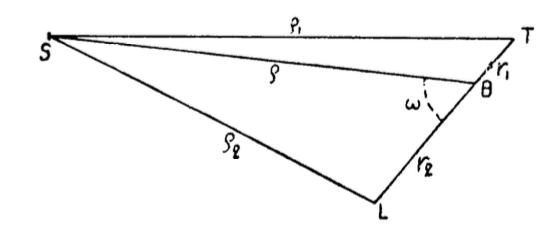
\includegraphics[width=0.48\textwidth]{21.png}
	\end{center}
	\vspace{-20pt}
	\caption{}
	\label{fig:noname_1}
	\vspace{-20pt}
\end{wrapfigure}

Солнце $S$ сообщает ускорения:
%
\begin{equation*}
\begin{aligned}
	& \text{Земле:} & f\cdot\frac{S}{\rho{_1}^2} & \text{ по направлению } & TS
	\\
	& \text{Луне:} & f\cdot\frac{S}{\rho{_2}^2} & \qquad \text{>>} \qquad \text{>>} \qquad & LS
\end{aligned}
\end{equation*}
%
вследствие чего точка $\Theta$ имеет ускорения:
%
\begin{equation*}
\begin{aligned}
	& \frac{T}{T+L} \cdot f \cdot \frac{S}{\rho{_1}^2} & \text{ по направлению, параллельно } & TS
	\\
	&  \frac{L}{T+L} \cdot f \cdot \frac{S}{\rho{_2}^2} & \text{>>} \qquad\qquad\qquad\text{>>} \qquad\qquad \text{>>} \qquad & LS
\end{aligned}
\end{equation*}

Ускорения Солнца, происходящие от притяжения Земли и Луны, соответственно, суть:
%
\begin{equation*}
\begin{aligned}
	& f\cdot\frac{T}{\rho{_1}^2} & \text{ по направлению } & ST
	\\
	& f\cdot\frac{L}{\rho{_2}^2} & \qquad\text{>>} \qquad\qquad\text{>>} \qquad & SL
\end{aligned}
\end{equation*}
%
поэтому ускорения точки $\Theta$ относительно точки $S$ будут:
%
\begin{equation*}
\begin{aligned}
	& \omega_1=f \cdot \frac{\left(S+T+L\right)}{T+L} \cdot \frac{T}{\rho{_1}^2} \text{ по направлению параллельно} & TS
	\\
	& \omega_2=f \cdot \frac{S+T+L}{T+L} \cdot \frac{L}{\rho{_2}^2} \qquad\text{>>} \qquad\text{>>} \qquad\text{>>} & LS
\end{aligned}
\end{equation*}
%
Разлагая эти ускорения, соответственно, по направлениям $\Theta S$ и $\Theta L$, получим, как легко видеть из подобия показанных на рис. \ref{fig:noname_2} и \ref{fig:noname_3} треугольников:
%
\begin{equation*}
\begin{aligned}
	& \omega_1' = \omega_1 \cdot \frac{\rho}{\rho_1} & \text{ по направлению } & \Theta S
	\\
	& \omega_1'' = \omega_1 \cdot \frac{r_1}{\rho_1} & \text{ >> } \qquad \text{ >> } & \Theta L
	\\
	& \omega_2' = \omega_2 \cdot \frac{\rho}{\rho_2} & \text{ >> } \qquad \text{ >> } & \Theta S
	\\
	& \omega_2'' = \omega_2 \cdot \frac{r_2}{\rho_2} & \text{ >> } \qquad \text{ >> } & L \Theta
\end{aligned}
\end{equation*}
%
\begin{figure}[H]
	\centering
	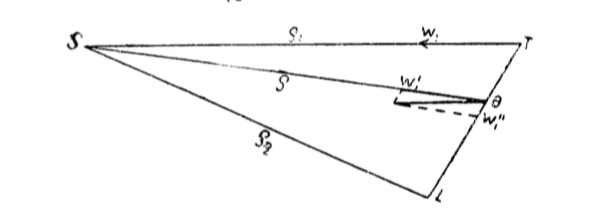
\includegraphics{22.png}
	\caption{}
	\label{fig:noname_2}
\end{figure}
%
получим для ускорений точки $\Theta$ слагающие:
%
\begin{equation*}
\begin{aligned}
	W_1 = \omega_1' + \omega_2' = f \cdot \frac{S+T+L}{T+L} \cdot
		\left[
			T \cdot \displaystyle \frac{\rho}{\rho{_1}^3} + L \cdot \displaystyle \frac{\rho}{\rho{_2}^3}
		\right] \text{ по } \Theta S
	\\
	W_2 = \omega_1'' - \omega_2'' = f \cdot \frac{S+T+L}{T+L} \cdot
		\left[
			T \cdot \displaystyle \frac{r_1}{\rho{_1}^3} - L \cdot \displaystyle \frac{r_2}{\rho{_2}^3}
		\right] \text{ по } \Theta L \\
\end{aligned}
\end{equation*}
%
\begin{figure}[H]
	\centering
	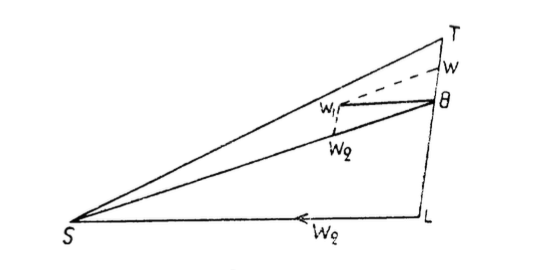
\includegraphics{23.png}
	\caption{}
	\label{fig:noname_3}
\end{figure}

Заменив $r_1$ и $r_2$ их выражениями \eqref{eq:1}, имеем:

$W_1 = f \cdot \displaystyle \frac{S+T+L}{T+L} \cdot \rho \cdot \left[ \displaystyle \frac{T}{\rho{_1}^3} + \displaystyle \frac{L}{\rho{_2}^3} \right]$ по направлению $\Theta S$

$W_2 = f \cdot \displaystyle \frac{S+T+L}{(T+L)^2} \cdot T \cdot L \cdot r 
\left\lfloor \frac{1}{\rho{_1}^3} - \frac{1}{\rho{_2}^3} \right\rfloor$ по направлению $\Theta L$

Но
%
\begin{equation*}
	\begin{aligned}
		&\rho{_1}^2 = \rho^2 + 2\rho \cdot \frac{L}{T+L} \cdot r\cos\omega+\left(\frac{L}{T+L} \cdot r \right)^2 \\
		&\rho{_2}^2 = \rho^2-2\rho \cdot \frac{T}{T+L} \cdot r\cos\omega+\left(\frac{T}{T+L}r\right)^2
	\end{aligned}
\end{equation*}
%
следовательно:
%
\begin{equation*}
\begin{aligned}
& \frac{1}{\rho{_1}^3} = \frac{1}{\rho^3}
	\left[
		1+3\frac{L}{T+L}\cos\omega+
		\left(
			\frac{L}{T+L}r
		\right)^2
		\left(
			-\frac{3}{2}+\frac{15}{2}\cos^2\omega
		\right) + \dots
	\right]
	\\
& \frac{1}{\rho{_2}^3}=\frac{1}{\rho^3}
	\left[
		1+3\frac{T}{T+L}\cos\omega+
		\left(
			\frac{T}{T+L}r
		\right)^2
		\left(
			-\frac{3}{2}+\frac{15}{2}\cos^2\omega
		\right)
		+ \dots
	\right]
\end{aligned}
\end{equation*}
%
Подставляя эти выражения, имeем:
%
\begin{equation*}
\begin{aligned}
	& W_1=f \cdot \frac{S+T+L}{\rho^2}
		\left[
			1+\frac{T \cdot L}{\left(T+L\right)^2} \cdot \frac{r^2}{\rho^2}
			\left(
				-\frac{3}{2}+\frac{15}{2}\cos^2\omega
			\right) + \dots
		\right]
	\\
	& W_2=f \cdot \frac{S+T+L}{\rho^2}
		\left[
			-3 \cdot \frac{T \cdot L}{(T+L)^2} \cdot \frac{r^2}{\rho^2}\cos\omega+\cdots
		\right]
\end{aligned}
\end{equation*}

Но отношения
%
\[\frac{T}{T+L} \approx \frac{1}{80}; \qquad \frac{r}{\rho} \approx \frac{1}{400}; \qquad \left(\frac{r}{\rho}\right)^2 = \frac{1}{160000}\]
%
поэтому будет
%
\[\frac{T \cdot L}{\left(T+L\right)^2} \cdot \frac{r^2}{\rho^2} \approx \frac{1}{12800000}\]
%
и члены, содержащие этот множитель, могут быть отброшены, так что будет:
%
\begin{equation*}
\begin{aligned}
	& W_1=f \cdot \frac{S+T+L}{\rho^2} \text{ по направлению } \Theta S
	\\
	& W_2=0  \text{ по направлению } \Theta L
\end{aligned}
\end{equation*}


Отсюда следует, что точка $\Theta$ движется вокруг Солнца по эллиптической орбите по законам Кеплера.

Рассмотрим теперь ускорение Луны по отношению к Земле, для чего к ускорениям, сообщаемым Луне Солнцем и Земплёю, надо присовокупить ускорение, равное и противоположное ускорению Земли, происходящему от действия Солнца и Луны. Поступив подобно предыдущему, получим:
%
\[f \cdot \frac{T+L}{r^2} + f \cdot S \left[\frac{r_2}{\rho{_2}^2} + \frac{r_1}{\rho{_3}^3}\right] \text{ по направлению $L\Theta$}\]
%
\[f \cdot S \cdot \rho \left[\frac{1}{\rho{_2}^3} - \frac{1}{\rho{_1}^3}\right] \text{ параллельно } \Theta S\]
%
положим:
%
\[T+L=\mu; S=M\]

% чтобы список иллюстраций и таблиц были на одной странице (нагуглил :-))
\listoffigures
\begingroup
\let\clearpage\relax
\listoftables
\endgroup

\end{document}
